\documentclass[
	12pt,				% tamanho da fonte
	openright,			% capítulos começam em pág ímpar (insere página vazia caso preciso)
	oneside,			% para impressão em recto e verso. Oposto a oneside
	a4paper,			% tamanho do papel. 
	english,			% idioma adicional para hifenização
	french,				% idioma adicional para hifenização
	spanish,			% idioma adicional para hifenização
	brazil				% o último idioma é o principal do documento
	]{abntex2}

\usepackage{lmodern}			% Usa a fonte Latin Modern			
\usepackage[T1]{fontenc}		% Selecao de codigos de fonte.
\usepackage[utf8]{inputenc}		% Codificacao do documento (conversão automática dos acentos)
\usepackage{indentfirst}		% Indenta o primeiro parágrafo de cada seção.
\usepackage{color}				% Controle das cores
\usepackage{graphicx}			% Inclusão de gráficos
\usepackage{microtype} 			% para melhorias de justificação
\usepackage{transparent}
\usepackage{eso-pic}
\usepackage{amsthm,amsfonts}
\usepackage{float}
\usepackage{multirow}
\usepackage[table,xcdraw]{xcolor}
\usepackage{longtable}
\usepackage{lipsum}				% para geração de dummy text
%\usepackage[brazilian,hyperpageref]{backref}	 % Paginas com as citações na bibl
\usepackage[alf]{abntex2cite}	% Citações padrão ABNT
\usepackage{xcolor}
\usepackage{scalefnt}

\usepackage[font=small]{caption}     %% make caption in normal size
\usepackage{etoolbox}
\AtBeginEnvironment{longtabu}{\footnotesize}{}{}   %% change all longtabu content to foot note size

\definecolor{verde}{rgb}{0,0.5,0}
\usepackage{listings}
\lstset{
  language=C++,
  basicstyle=\ttfamily\small,
  keywordstyle=\color{blue},
  stringstyle=\color{verde},
  commentstyle=\color{red},
  extendedchars=true,
  showspaces=false,
  showstringspaces=false,
  numbers=left,
  numberstyle=\tiny,
  breaklines=true,
  backgroundcolor=\color{green!10},
  breakautoindent=true,
  captionpos=b,
  xleftmargin=0pt,
}


\titulo{Processo Agroindustrial de Processamento de Cacau}
\autor{Caio Henrique Silva Souza 99131\\Eduardo Favoretto Vale Bom 108139\\Gabriel Rodrigues Munhoz 106802\\João Vítor Batistão 108074}
\local{Maringá, PR}
\data{01.02.2022}
\orientador{}
\coorientador{}
\instituicao{%
  Universidade Estadual de Maringá - UEM
  \par
  Departamento de Engenharia de Produção - DEP}
\tipotrabalho{Tese (Doutorado)}
\preambulo{}

\definecolor{blue}{RGB}{41,5,195}

\makeatletter
\hypersetup{
     	%pagebackref=true,
	pdftitle={\@title}, 
	pdfauthor={\@author},
    	pdfsubject={\imprimirpreambulo},
	pdfcreator={LaTeX with abnTeX2},
	pdfkeywords={abnt}{latex}{abntex}{abntex2}{trabalho acadêmico}, 
	colorlinks=true,       		% false: boxed links; true: colored links
    	linkcolor=black,          	% color of internal links
    	citecolor=blue,        		% color of links to bibliography
    	filecolor=magenta,      		% color of file links
	urlcolor=blue,
	bookmarksdepth=4
}

\setlength{\parindent}{1.3cm}

\setlength{\parskip}{0.2cm}  % tente também \onelineskip

\makeindex

%\usepackage{fancyhdr}
%\fancyhead{}
%\fancyfoot{}
%\lhead{Processo Agroindustrial de Processamento de Cacau}
%\rhead{Processo Agroindustrial de Processamento de Cacau}

\AddToShipoutPicture{
\put(0,0){
\parbox[b][\paperheight]{\paperwidth}{%
\vfill
\centering
{\transparent{0.1}\includegraphics[scale=1.4]{../../Pictures/logoUEM.jpg}    }%
\vfill}}}



%\graphicspath{{../Pictures}}
\begin{document}

\begin{minipage}[c][0cm][c]{0cm} % a primeira minipágina tem uma altura de 1.5cm e uma largura de 3cm.

\centering


\includegraphics[scale=0.45]{../../Pictures/uem-modelo-04.png}  
\end{minipage}

\selectlanguage{brazil}

\frenchspacing 

% \pretextual

\imprimircapa


% ---
% RESUMOS
% ---

%\setlength{\absparsep}{18pt} % ajusta o espaçamento dos parágrafos do resumo
%\begin{resumo}
 
 
% \textbf{Palavras-chave}: latex. abntex. editoração de texto.
%\end{resumo}


% ---
% inserir o sumario
% ---
\pdfbookmark[0]{\contentsname}{toc}
\tableofcontents*
\cleardoublepage

% ----------------------------------------------------------
% ELEMENTOS TEXTUAIS
% ----------------------------------------------------------
\textual

\chapter{Introdução}
%\pagestyle{fancy}

\section{Contextualização do Tema}

O cacau é um fruto da espécie \textit{Theobroma cacao L.} que possui origem na região amazônica e seu uso, segundo arqueólogos equatorianos e franceses, já era realizado há cerca de 5.500 anos pelos povos amazônicos \cite{2}. No entanto, foi no século XVII que acabou se tornando um produto agrícola e cultivado em diferentes locais da América do Sul e Central devido a disseminação do cultivo pelos espanhóis, e posteriormente se expandindo aos poucos pelo mundo. \cite{1} 

Existem 6 principais produtos a partir do fruto de cacau: mel, polpa, nibs, chocolate, manteiga e cacau em pó, além da própria amêndoa do cacau e casca que também pode ser comercializada de uma forma menos processada. A maior parte desses produtos são voltados para o setor alimentício, no entanto é possível verificar aplicações também no setor cosmético e no setor de geração de energia. \cite{5}

Com mais da metade da produção nacional, 62$\%$, o sul da Bahia é a principal região produtora de cacau, seguida pela região norte do Brasil com 34$\%$ e o restante da produção, 4$\%$, espalhada pelo país \cite{1}. O Brasil é o 7º maior produtor do mundo e segundo o Instituto Brasileiro de Geografia Estatística (IBGE) o Brasil produziu em torno de 310 mil tonaledas. \cite{3} 

\section{Objetivos}

\subsection{Objetivo Geral}

Estudar o processamento de cacau na agroindústria, mais especificamente a produção de chocolate, abrangendo desde a parte normativa do setor, até o entendimento do mercado do produto em questão e as análises técnicas dos processos.

\subsection{Objetivos Específicos}

\begin{itemize}
\item Estudar o mercado, normas regulatórias, oportunidades e desafios do setor.
\item Realizar o mapeamento dos processos de uma produção de chocolate desde o recebimento do fruto até a embalagem, estoque e distribuição do produto final.
\item Calcular os balanços de massa e energia que são inerentes ao processo de produção.
\end{itemize}

\newpage
\chapter{Planejamento Estratégico de Produtos}
%\pagestyle{fancy}

\section{Definir escopo da revisão do PEN}

Nesta atividade do Item “Planejamento estratégico de Produtos”, visto que
não temos uma empresa “real” para o desenvolvimento do produto, portanto,
ela não possui um planejamento estratégico, é preciso definir algumas
questões. Assim, nessa atividade devem ser definidos pelo menos:
Missão
Visão
Valores
Segmento de mercado
Alguns objetivos e metas a serem alcançadas a longo prazo pela empresa
(estratégias).
No mínimo três ideias de produtos para seu portfólio (cada um terá uma
minuta breve, mas somente um será desenvolvido).


\section{Planejar atividades para a revisão do PEN}

Apresentar o planejamento de como se dará as próximas atividades do Item.

\section{Consolidar informações sobre tecnologia e mercado}




\section{Revisar o PEN}


Nesta atividade poderá ser revisto o que foi definido no Item 2.1 pela equipe
com as informações obtidas na atividade 2.3. Apresentando, então, as
possíveis alterações ou a manutenção do que foi previamente definido.

Nesta atividade os produtos definidos na atividade 2.1 podem ser analisados
baseados em técnicas que utilizam critérios relacionados a estratégia da
empresa.

\section{Analisar o portfólio de produtos da empresa}

\section{Propor mudanças no portfólio de produtos}

\section{Verificar a viabilidade do portfólio de produtos}

Aqui fica dispensada a atividade de “Avaliar a viabilidade econômica do
portfólio de projetos”.

\section{Decidir o início do planejamento de um dos produtos do portfólio}

\newpage
\chapter{Planejamento do Projeto}
%\pagestyle{fancy}

\section{Definir interessados do projeto}

\section{Definir escopo do produto}

\section{Definir escopo do projeto}

\section{Detalhar o escopo do projeto}

\section{Adaptar o modelo de referência}

\section{Definir atividades e sequência}

\section{Preparar cronograma}

\section{Avaliar riscos}

\section{Preparar orçamento do projeto}

\section{Analisar a viabilidade econômica do projeto}

\section{Definir indicadores de desempenho}

\section{Definir plano de comunicação}

\section{Planejar e preparar aquisições}

\section{Preparar plano de projeto}


\newpage
\chapter{Projeto Informacional}
%\pagestyle{fancy}

\section{Revisar e atualizar o escopo do produto}

\section{Detalhar ciclo de vida do produto e definir seus clientes}

\section{Identificar os requisitos dos clientes do produto}

\section{Definir os requisitos do produto}

\section{Definir especificações-meta do produto}


\newpage
\chapter{Projeto Conceitual}
%\pagestyle{fancy}

\section{Modelar funcionalmente}

Como função global, o filtro de água para pets, tem como principal objetivo retirar as impurezas da água, tornando-a assim, própria para o consumo.

\begin{figure}[H]
\begin{center}
\caption{Funcionamento do produto de forma resumida}
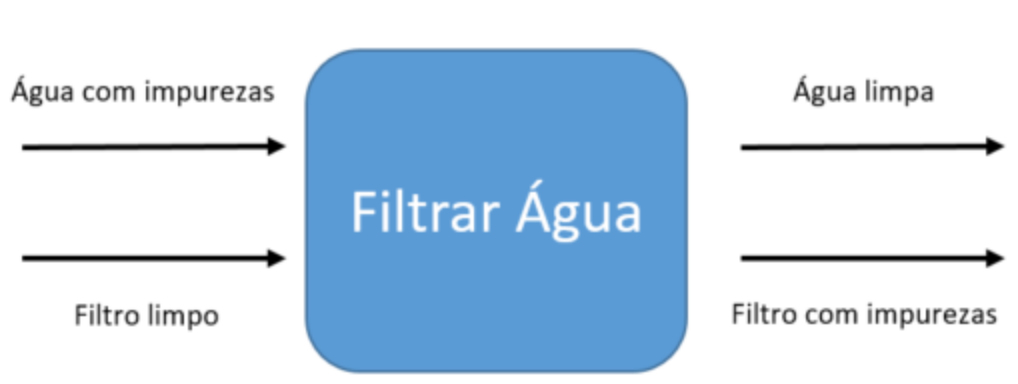
\includegraphics[scale=0.3]{/home/grmunhoz/Documents/Munhoz/University/Pictures/agua.png} 
\label{figetapas}
\legend{Fonte: Autoria Própria}
\end{center}
\end{figure}

Como entrada do nosso processo de funcionamento, temos a água contendo impurezas, e a utilização de um filtro limpo, que deve ser trocado de seis em seis meses. Como saída, temos a água limpa, própria para o consumo dos pets, e o filtro com as impurezas retiradas da água.

\begin{figure}[H]
\begin{center}
\caption{Funcionamento do produto detalhado}
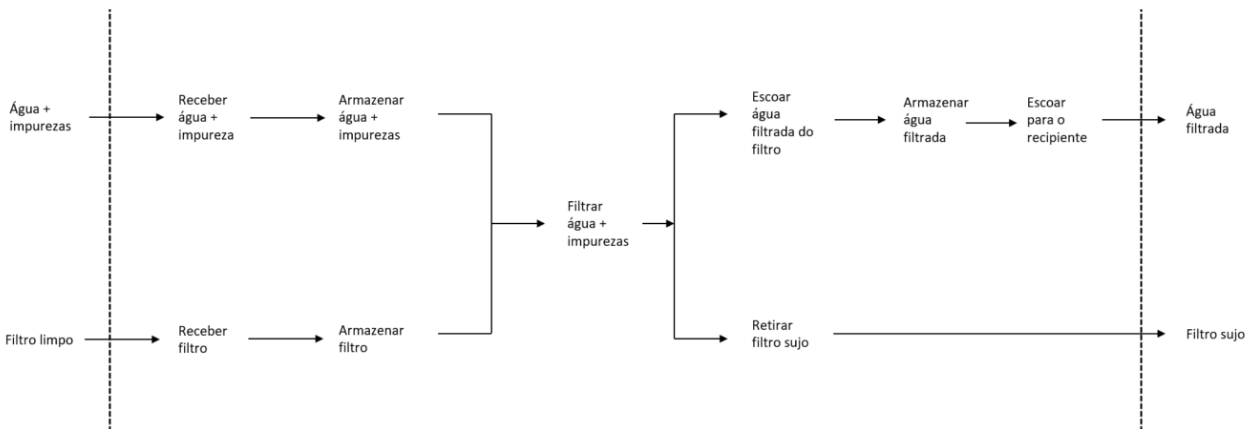
\includegraphics[scale=0.5]{/home/grmunhoz/Documents/Munhoz/University/Pictures/fluxo.png} 
\label{figetapas}
\legend{Fonte: Autoria Própria}
\end{center}
\end{figure}


\section{Desenvolver princípios de soluções para as funções}

Para o desenvolvimento dos princípios de soluções para as funções, foi utilizado o método de criatividade da matriz morfológica. A metodologia consiste no desdobramento de um problema complexo e partes mais simples, e combinando as diferentes funções, com os princípios de solução, busca a melhor combinação para o desenvolvimento do produto.


\section{Desenvolver alternativas de solução}

A metodologia foi aplicada para resolver dois principais problemas no desenvolvimento do produto. O primeiro, como seria a inserção da água no início do processo de uso. O segundo problema, como seria armazenada a água após a filtragem, ou seja, como o pet beberia a água filtrada. Com a aplicação da metodologia, chegamos em três principais alternativas para a solução do problema:

\begin{figure}[H]
\begin{center}
\caption{Alternativas de solução}
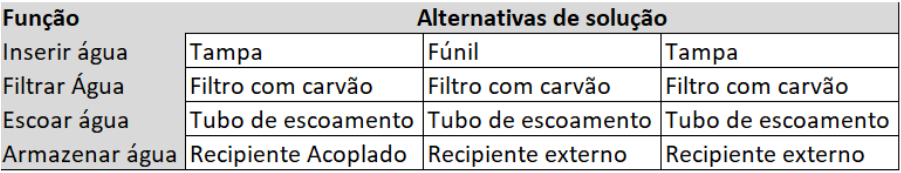
\includegraphics[scale=0.65]{/home/grmunhoz/Documents/Munhoz/University/Pictures/alternativas.png} 
\label{figetapas}
\legend{Fonte: Autoria Própria}
\end{center}
\end{figure}

\section{Definir arquitetura}

Como será especificado nos próximos tópicos, a alternativa de solução escolhida foi o produto com tampa e com o recipiente acoplado:

\begin{figure}[H]
\begin{center}
\caption{Alternativas de solução}
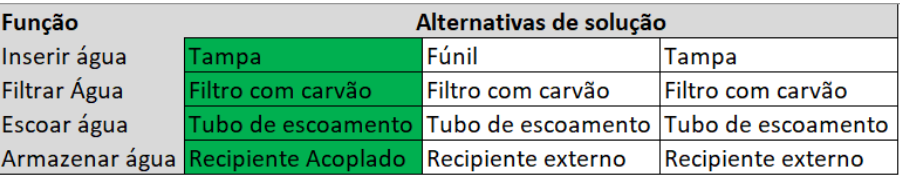
\includegraphics[scale=0.65]{/home/grmunhoz/Documents/Munhoz/University/Pictures/funcao.png} 
\label{figetapas}
\legend{Fonte: Autoria Própria}
\end{center}
\end{figure}


A escolha da tampa foi por conta da praticidade quando necessário o reabastecimento. O recipiente acoplado, acreditamos que é adaptável a todas as raças e tamanhos de cães e gatos, e por isso, torna o produto completo, sem necessidade da compra de um recipiente a parte.

\section{Analisar SSCs}

A solução escolhida anteriormente é composta de pequenos suportes com adesivos para fixação em paredes ou superfícies lisas e bocal com tubo para utilização em bebedouros separados e com adaptador de bocal para uso como um cantil suspenso.

\begin{figure}[H]
\begin{center}
\caption{Desenho do produto com as dimensões}
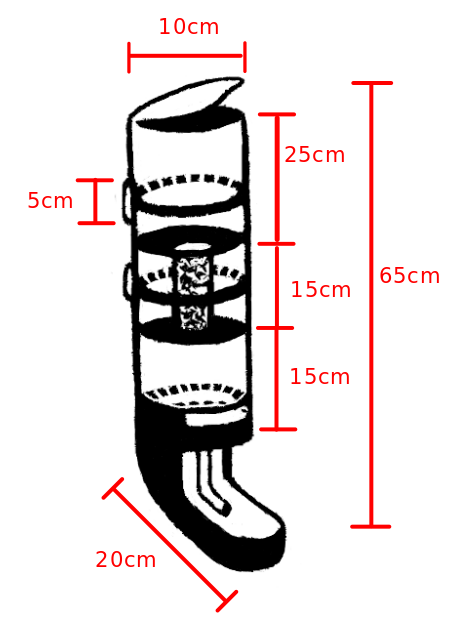
\includegraphics[scale=0.7]{/home/grmunhoz/Documents/Munhoz/University/Pictures/draft2.1.png} 
\label{figetapas}
\legend{Fonte: Autoria Própria}
\end{center}
\end{figure}


O produto possui no total 65 cm de altura e consegue armazenar um pouco mais de 3 litros de água devido seu diâmetro de 10 cm. O bocal possui 7cm de altura e um diâmetro de apenas 1 cm, já o acessório de cantil de água possui 10 cm de altura e 20 cm de comprimento sendo sua largura do mesmo diâmetro do corpo do produto. 

O material predominante no produto é o plástico polipropileno reciclado. Esse termoplástico é utilizado em toda a estrutura do bebedouro, inclusive no bocal e no acessório de cantil. Enquanto o filtro é um conjunto de carvão ativado envolto por plástico também polipropileno. Além desses materiais também se encontram no produto pequenas partes de metal para encaixes e adesivos nos suportes para fixação em superfícies.


\section{Definir ergonomia e estética}

A ergonomia do produto foi pensada tanto para a utilização pelos pets assim como para a manutenção do equipamento pelos tutores. Foi projetado um sistema de suporte de fácil instalação e que pode ser utilizado em diversos tipos de superfícies. Dessa forma se o cliente utiliza um bebedouro elevado, o produto desenvolvido consegue ficar na altura ideal e caso o dono estiver usando o acessório de cantil suspenso os animais não precisam se abaixar muito para beber a água. 

Outro ponto importante abordado em relação a ergonomia foi a manutenção do filtro e o preenchimento com água. A tampa primeiramente possui uma borda lateral que facilita a abertura e o preenchimento com água, já que a tampa pode ser aberta por completo por meio de uma pequena dobradiça. Além disso, o diâmetro do tubo de armazenamento foi projetado para que uma pessoa consiga manusear e desrosquear o filtro de forma simples, facilitando assim o processo de troca que deve ocorrer de 6 em 6 meses. 

O processo de limpeza também foi levado em conta para o desenvolvimento da estética e do formato do aparelho. Pensando nisso, o produto consegue ser desmontado de forma fácil e a limpeza pode ser feita rapidamente.

Com relação a estética final, o produto possui várias possibilidades de cores: azul, cinza, vermelho, verde, branco e preto, no entanto, essas cores são apenas utilizadas nos detalhes do bebedouro como os suportes para o bebedouro em si, o suporte para o filtro interno, as tampas e o acessório de cantil. O formato é cilíndrico e possui as arestas arredondadas. 


\section{Definir parcerias de co-desenvolvimento}

Para participar do desenvolvimento do produto foram definidas parcerias no mercado pet, no segmento de termoplásticos e também no setor de embalagens. Entre eles se encontram estabelecimentos varejistas e atacadistas, como pet shops, fabricantes de embalagens e indústrias de injeção plástica. Além disso, também foram negociadas parcerias com canis e ONGs para validação do projeto e também para a divulgação do produto.

%\section{Definir plano macro de processo}

\newpage
\chapter{Projeto Detalhado}
%\pagestyle{fancy}

\section{Criar e detalhar itens e documentos}

No desenvolvimento desta fase, é realizada o descrição em forma de lista dos SSCs (Sistema, Subsistemas e componentes), além da codificação dos produtos, o desenho do mesmo e suas especificações iniciais.

Os SSCs do bebedouro são os seguintes:

\begin{itemize}
\item Sistema: Bebedouro filtrante para PETs
\item Subsistemas: Estrutura externa, adaptadores de bocal, filtro,compartimento secundário e recipiente final
\item Componentes: 
\subitem Estrutura externa: Plástico e apoio
\subitem Adaptadores de bocal: Hastes e garras
\subitem Filtro: Carvão ativado,  Quartzo, Dolomita e Alumina;
\subitem Recipiente: Filete anterior ao recipiente e o próprio recipiente
\end{itemize}

\begin{figure}[H]
\begin{center}
\caption{Detalhamento dos itens}
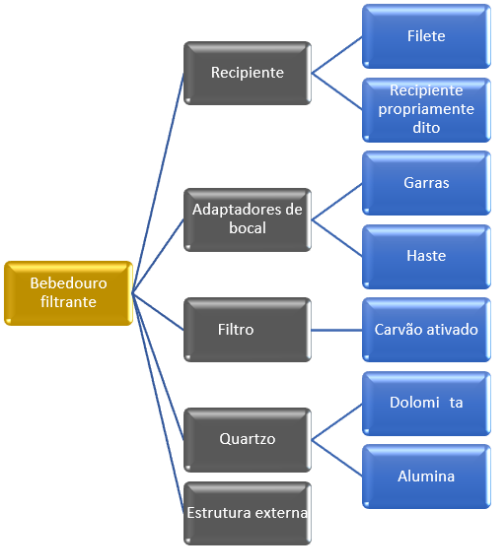
\includegraphics[scale=0.6]{/home/grmunhoz/Documents/Munhoz/University/Pictures/arvore.png} 
\label{figetapas}
\legend{Fonte: Autoria Própria}
\end{center}
\end{figure}

As especificações das tolerâncias são levantadas pelos fornecedores e mantém um padrão considerável e como são poucos componentes com possibilidade de variação está etapa é simples e direta, tendo uma possibilidade de variação no tamanho dos materiais injetáveis em  +/- 0,1 e além disso nenhum tipo de defeito é tolerado, bem como riscos, manchas e raspões.

\section{Decidir fazer ou comprar SSCs}

Para o desenvolvimento do produto, será necessário comprar os componentes como o plástico pronto para realizar a injeção, os componentes do filtro(Carvão ativado,  Quartzo, Dolomita e Alumina), e as hastes de ferro. Com isso, será feito internamente na fábrica a injeção plástica para a produção da estrutura externa do bebedouro, a estrutura do filtro e o recipiente final.

\begin{itemize}
\item Estrutura externa: Plástico e apoio (Fabricar)
\item Adaptadores de bocal: Hastes e garras (Comprar)
\item Filtro: Carvão ativado,  Quartzo, Dolomita e Alumina (Comprar)
\item Recipiente: Filete anterior ao recipiente e o próprio recipiente (Fabricar)
\end{itemize}


\section{Planejar processo de fabricação e montagem}

Os processos de fabricação macro são os seguintes:

\begin{itemize}
\item Injeção plástica da estrutura externa do bebedouro;
\item Injeção plástica da estrutura do filtro;
\item Injeção plástica do recipiente final do bebedouro;
\item Montagem de todas as partes separadas do bebedouro: Recipiente, Filtro, estrutura externa e adaptadores
\end{itemize} 
	
Para a injeção, o procedimento é simples, pois é utilizada um mesmo modelo de máquina injetora com moldes diferentes para cada tipo de injeção(recipiente e estruturas externas);

Para a montagem o procedimento será o seguinte:
\begin{figure}[H]
\begin{center}
\caption{Processo de montagem}
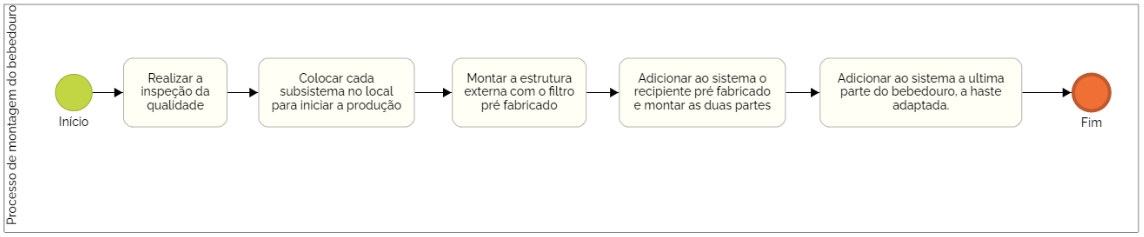
\includegraphics[scale=0.5]{/home/grmunhoz/Documents/Munhoz/University/Pictures/processo.png} 
\label{figetapas}
\legend{Fonte: Autoria Própria}
\end{center}
\end{figure}

\section{Projetar recursos de fabricação}

Já os insumos necessários para o o será fabricado internamente na indústria, como comentado anteriormente, são o plástico injetável e a matéria prima para a produção do filtro. 

Para a injeção, algumas matérias primas específicas são necessárias, e para isso existem muitas possibilidades:

\begin{itemize}
\item Injeção de plástico em ABS
\item Injeção de plástico em Nylon
\item Injeção de plástico em Poliestireno
\item Injeção de plástico em Polietileno
\item Injeção de plástico em Polipropileno
\item Injeção de plástico em Poliuretano
\item Injeção de plástico em PVC
\end{itemize}

No entanto, para a produção do produto só serão utilizados alguns desses tipos de injeção.

Os plástico para serem injetados necessitam estar em pedaços, para assim serem colocados nas máquina e assim a injeção aconteça de forma efetiva. a seguir será apresentado em imagem como são os plásticos antes de serem injetados:

\begin{figure}[H]
\begin{center}
\caption{Plásticos para injeção}
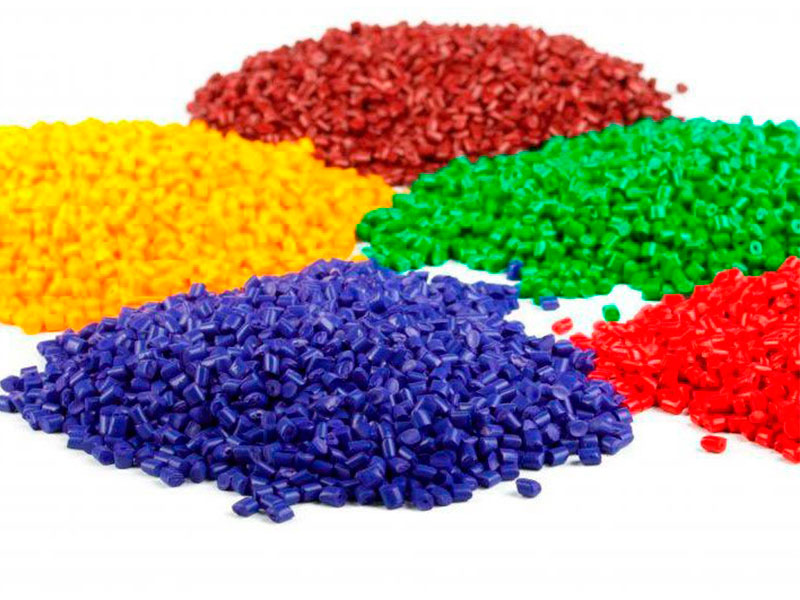
\includegraphics[scale=0.3]{/home/grmunhoz/Documents/Munhoz/University/Pictures/plastico.jpg} 
\label{figetapas}
\legend{Fonte: Google}
\end{center}
\end{figure}


\section{Avaliar itens e documentos}

Para um produto entrar em circulação e poder ser comercializado livremente é necessário estar em consonância com as normas estabelecidas por lei.

Para um produto como um bebedouro, todas as normas estabelecidas foram levadas em consideração desde o início do desenvolvimento do projeto e o produto está dentro de todas as normas existentes.


\section{Otimizar produto e processo}

Como evidenciado no tópico anterior a conformidade com todas as normas vigentes tanto de produção, quanto de utilização, tipo de consumidor, materiais e descarte; foram tomadas como pré-requisitos para o desenvolvimento do produto.

Assim, após a verificação anterior podemos constatar que o produto atende a todas as exigências normativas referentes a sua fabricação, distribuição e uso. Por isso não foi necessária nenhuma otimização nesse sentido.


\section{Criar material de suporte do produto}

O filtro a ser desenvolvido é um item de utilização simples, por isso não foi necessário o desenvolvimento de materiais de suporte complexos. Todavia junto da embalagem do item será enviado um folheto com instruções básicas de utilização e conservação, assim como descrição do item e informações para que os consumidores façam um descarte correto do produto após o fim da sua vida útil.

As informações de utilização e conservação terão como objetivo informar ao consumidor o uso correto do produto além de ações necessárias para sua conservação durante o ciclo de vida do produto e o bom funcionamento.

O material de suporte também contará com uma breve descrição do produto, partes e materiais que compõem o produto, para que o consumidor entenda o produto e esteja ciente da sua composição.

Além disso, contará com as informações para descarte correto do item, seguindo a missão da empresa de popularizar no Brasil a utilização de materiais alternativos e ecológicos em produtos inovadores.

\section{Projetar embalagem}

A embalagem desenvolvida foi pensada para proteger o produto principalmente de danos mecânicos que podem sofrer ao longo do transporte e possibilitar sua distribuição para todo o país. Por não se tratar de um objeto frágil a embalagem será composta basicamente por uma embalagem de papelão onde o produto será colocado dentro e o espaço vazio dentro da embalagem será preenchido por um material chamado Bio Pack.

O Bio Pack é uma espécie de espuma de origem vegetal que pode ser usada para preencher embalagens e proteger objetos. Com composição 100$\%$ biodegradável, o Bio Pack cumpre a função de proteção (comumente desempenhada pelo plástico-bolha), com a vantagem de não agredir o meio ambiente.

Para comportar o nosso produto a embalagem tem 70cm de comprimento, 30 cm de largura e 20 cm de altura.

\begin{figure}[H]
\begin{center}
\caption{Dimensões da embalagem de papelão}
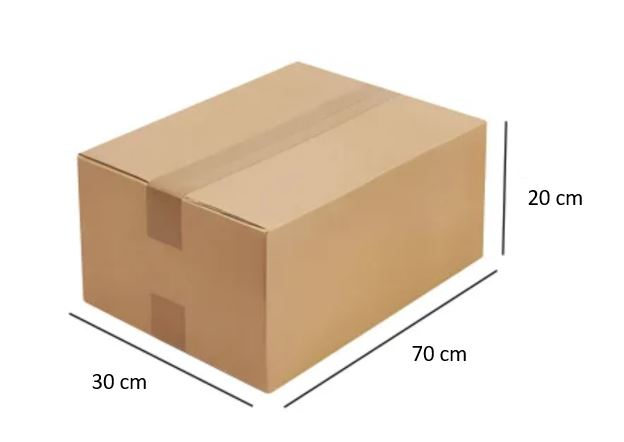
\includegraphics[scale=0.7]{/home/grmunhoz/Documents/Munhoz/University/Pictures/embalagem.JPG} 
\label{figetapas}
\legend{Fonte: Autoria Própria}
\end{center}
\end{figure}

\begin{figure}[H]
\begin{center}
\caption{Bio pack}
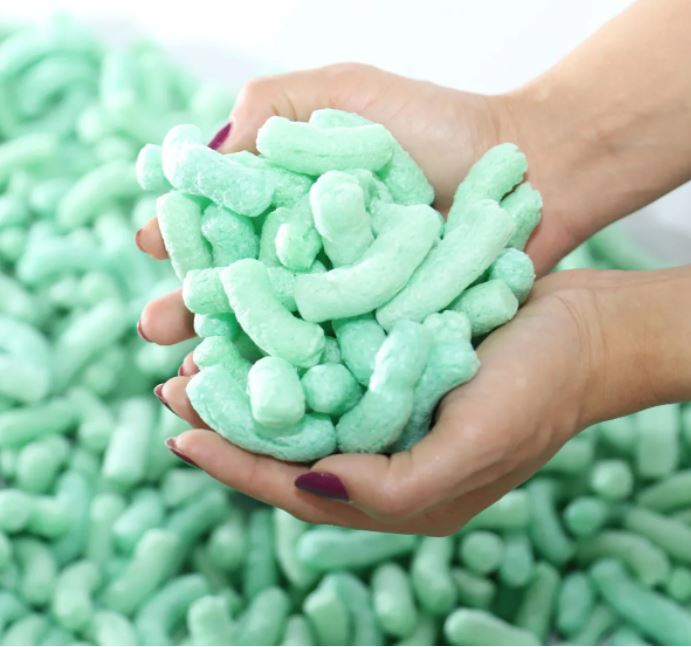
\includegraphics[scale=0.5]{/home/grmunhoz/Documents/Munhoz/University/Pictures/bio pack.JPG} 
\label{figetapas}
\legend{Fonte: Google}
\end{center}
\end{figure}


\section{Planejar fim de vida de produto}

A última etapa do ciclo de vida do produto é justamente o fim da sua vida útil e o descarte ou reutilização. Para nossa empresa o compromisso com o meio ambiente através da reutilização dos produtos ou descarte correto é imprescindível.

Dessa forma para esse produto será disponibilizado ao consumidor um departamento comercial onde a própria empresa receberá de volta o item após o fim da sua vida útil (6 meses) para reutilizar partes dele, já que a empresa conta com um portfólio de produtos ecológicos e reciclados, e também será feito o descarte de produtos que não podem ser reutilizados, como o filtro de carvão ativado.

Caso o consumidor opte por ele mesmo fazer o descarte do material ele deve seguir algumas recomendações. Conforme a Norma Brasileira da ABNT, NBR 10004, os resíduos são classificados nas seguintes classes:

\begin{itemize}
\item Classe I: Perigosos;
\item Classe II: Não perigosos;
\subitem A: Não inertes;
\subitem B: Inertes.
\end{itemize}

O elemento filtrante, que é o carvão ativado, é considerado resíduo Classe II A: Não Inertes. Isso significa que não se apresentam inflamáveis, corrosivos, tóxicos, patogênicos, e nem possuem tendência a sofrer uma reação química. E ainda, podem ter propriedades, tais como: biodegradabilidade, combustibilidade ou solubilidade em água.

Assim, os resíduos que possuem essa classificação podem ser descartados em lixos recicláveis, na lata indicada com a cor vermelha referente a lixo composto por componentes plásticos.

\begin{figure}[H]
\begin{center}
\caption{Lixeira de reciclagem}
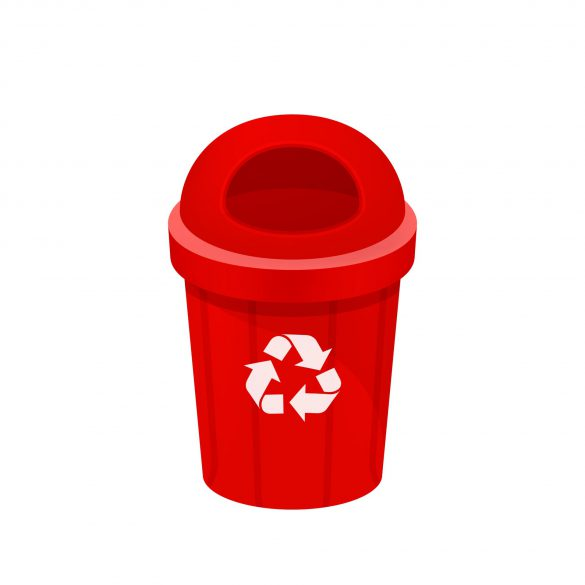
\includegraphics[scale=0.3]{/home/grmunhoz/Documents/Munhoz/University/Pictures/lixeira.JPG} 
\label{figetapas}
\legend{Fonte: Google}
\end{center}
\end{figure}

Além disso, o plástico, material que é feito o corpo do filtro, é reciclável e deve ser descartado em lixeiras específicas para esse material.

\section{Testar e homologar produto}

Após toda a trajetória de desenvolvimento do produto apresentado constatou-se que ele está em conformidade com os objetivos da empresa, sendo viável sua inclusão ao portfólio de produtos, além de se mostrar em conformidade com as necessidades e expectativas dos clientes e principalmente com todas as normas relacionadas.

Além disso, através do protótipo foi possível a realização de testes e comprovado que o item atende a todas as especificações de qualidade do projeto técnico do produto.

Dessa forma o produto está validado e pode ser homologado para iniciar sua fabricação e distribuição ao mercado consumidor.


\newpage
%\chapter{Prototipagem}
%\pagestyle{fancy}


%\newpage
\postextual

\bibliography{referencias}

%\begin{anexosenv}

%\chapter{Código utilizado no software EMSO}

%\begin{lstlisting}
%\end{lstlisting}

%\end{anexosenv}

\end{document}
